\documentclass[twoside,twocolumn,9pt]{article}

\usepackage[super,sort&compress,comma]{natbib}
\usepackage[left=1.5cm, right=1.5cm, top=1.785cm,
bottom=2.0cm]{geometry}
\usepackage[english]{babel}
\usepackage[T1]{fontenc}
\usepackage{hyperref}
\usepackage{graphicx}
\graphicspath{{./figures}{../figures}}
\usepackage{xcolor}

%\usepackage{epstopdf}
\usepackage{epstopdf}
\author{Mateo Barria-Urenda, José Antonio Gárate}
\title{Thermodynamic characterization of the adsorption of amino acids
  onto pristine graphene and graphene oxide}
\date{}

\begin{document}

\maketitle

\abstract{}

\section{Introduction}

% Context

First synthesized in 2004 \cite{Novoselov_2004}, graphene has since
experienced an explosive growth in interest \cite{Randviir_2014}.  For
pristine graphene, it's interactions with other particles are mainly
due to Van der Waals forces and $\pi-\pi$ stacking. \cite{Zuo_2012} As
pristine graphene is chemically inert \cite{Eftekhari_2017} a
classical description of it is expected to suffice in simulations.
Multiple molecular dynamics studies on the interactions between
proteins and carbon based nanoparticles (CBNs) --such as graphene--
have been published \cite{Zheng_2003, Ge_2011, Zuo_2012, Chong_2015,
  Duan_2015, Shityakov_2015, Al_Qattan_2018,Puigpelat_2019,
  Gonz_lez_Durruthy_2020, Li_2020}

% Need

% Task

% Work


\section{Methods}

\subsection{Free Energy Methods}

The Helmholtz free energy of adsorption of an amino acid onto a
graphene layer ($\Delta A_{ads}$) can be obtained from the difference
in free energy of the Adsorbed and Free states:

\begin{equation}
\label{eq:Adsorption}
\Delta A^{ads} = A^{near} - A^{free}
\end{equation}

Where the near and free states are defined based on the reaction
coordinate $\xi(\mathbf{r})$. $\xi(\mathbf{r})$ depends on the
coordinates of the system ($\mathbf{r}$) and is equal to the distance
between the graphene layer and the $\alpha-$carbon of the amino acid
projected onto a vector normal to the graphene layer. For a graphene
layer prepared along the XY plane, this is equivalent to the distance
along the Z--axis. The cut-off ranges for the near and far states will
be defined based on the PMFs (potentials of mean force) along $\xi(\mathbf{r})$ of
the amino acids, which can be found in the supplementary materials
\textcolor{red}{TODO}.

The free energy of a state is related to the probability of the state
via:

\begin{equation}
\label{eq:A-from-p}
A^i = - k_B T \ln (p_i)
\end{equation}

Where $k_B$ is Boltzmann's constant and T is the
temperature. Replacing Eq.~(\ref{eq:A-from-p}) in
Eq.~(\ref{eq:Adsorption}) we get an expression to calculate the free
energy of adsorption from the probabilities of the near and free
states:

\begin{equation}
\label{eq:Aads-from-p}
\Delta A^{ads} = - k_B T \ln (\frac{p_{near}}{p_{free}})
\end{equation}

If the PMF along $\xi$ has been estimated for the discrete
states $\{\xi_1, \xi_2, ..., \xi_N \}$, the probability of a state
$\xi_{j}$ can be estimated with:

\begin{equation}
\label{eq:p-from-PMF}
p_{\xi_j} = \frac{e^{-\beta~\mathrm{PMF}(\xi_j)}}{\sum_{i=1}^N e^{-\beta~\mathrm{PMF}(\xi_i)}}
\end{equation}

where $\beta$ is the thermodynamic beta ($\frac{1}{k_{B}T}$). To
estimate the probability of a state with multiple possible $\xi$
values, the numerator is replaced with a sum over the individual
values of $\xi$. In this way, the probabilities of the adsorbed and
free states can be estimated with:

\begin{equation}
\label{eq:p-near}
p_{near} = \frac{\sum_{j \in near} e^{-\beta~\mathrm{PMF}(\xi_j)}}{\sum_{i=1}^N e^{-\beta~\mathrm{PMF}(\xi_i)}}
\end{equation}
\begin{equation}
\label{eq:p-free}
p_{free} = \frac{\sum_{j \in free} e^{-\beta~\mathrm{PMF}(\xi_j)}}{\sum_{i=1}^N e^{-\beta~\mathrm{PMF}(\xi_i)}}
\end{equation}

Replacing Eqs.~(\ref{eq:p-near})~and~(\ref{eq:p-free}) in
Eq.\~(\ref{eq:Aads-from-p}) we have an expression to calculate the
free energy of adsorption from a PMF of $\xi$, regardless of how the
PMF was obtained:

\begin{equation}
\label{eq:Aads-from-PMF}
\Delta A^{ads} = - k_B T \ln \left(\frac{\sum_{j \in near} e^{-\beta~\mathrm{PMF}(\xi_j)}}{\sum_{k \in free} e^{-\beta~\mathrm{PMF}(\xi_k)}}\right)
\end{equation}

or, equivalently:

\begin{equation}
\label{eq:Aads-from-PMF-p}
\Delta A^{ads} = - k_B T \ln \left(\frac{\sum_{j \in near} p_{\xi_j}}{\sum_{k \in free} p_{\xi_k}}\right)
\end{equation}

On the following sections, two different methods used to obtain a PMF along $\xi$ will be described.

\subsubsection{Umbrella Sampling}

Umbrella sampling\cite{Torrie_1977} was used to obtain the PMF along
reaction coordinate by sampling multiple windows along $\xi$. Each sample
was obtained from a simulation where the Hamiltonian included the
following potential:

\begin{equation}
\label{eq:umbrella-potential}
\mathcal{V}^{US}(\mathbf{r}, k^{US}, \xi^0) = \frac{1}{2}k^{US}[\xi^0
- \xi(\mathbf{r})]^2
\end{equation}

where $\xi^0$ is the center of the sampling window and $k^{US}$ is an
harmonic constant. For simulations of amino acids over pristine
graphene $\xi^0$ took values from 0.3 to 1.5 nm in 0.05 nm steps, while $k^{US}$ took
values from 1000 to 12000 [$kJ \cdot mol \cdot nm^2$] adjusted to
ensure a good overlap in the sampling of different windows while
retaining a high sampling of the window's center.

The biased samples of $\xi$ obtained from these windows were used
to obtain the unbiased PMF using an implementation of the Weighted Histogram Analysis
Method (WHAM)\cite{Kumar_1992, Kumar_1995} developed by
\citet{WHAM}. This implementation of WHAM outputs --in addition to the
free energy/probability along $\xi$-- the (dimensionless) free energy
of each window, $F_i$. Knowing the $F_i$ of every we can unbias our
samples of any property $T$, to get an average for the window:

\begin{equation}
\label{eq:WHAM-unbias}
\langle T(\xi') \rangle = \frac{\sum_i^{S} \sum_j^{N_i} T_{i, j}
  e^{-\beta[F_i - \mathcal{V}^{US}(\mathbf{r_j})]}
  \delta \xi_{i, j}}{\sum_i^{S} \sum_j^{N_i}
  e^{-\beta[F_i - \mathcal{V}^{US}(\mathbf{r_j})]}
  \delta \xi_{i, j}}
\end{equation}

where



%\subsubsection{Well-Tempered Multiple Walker Metadynamics}

\subsection{Molecular Dynamics Simulation}

\begin{figure}[htbp]
\centerline{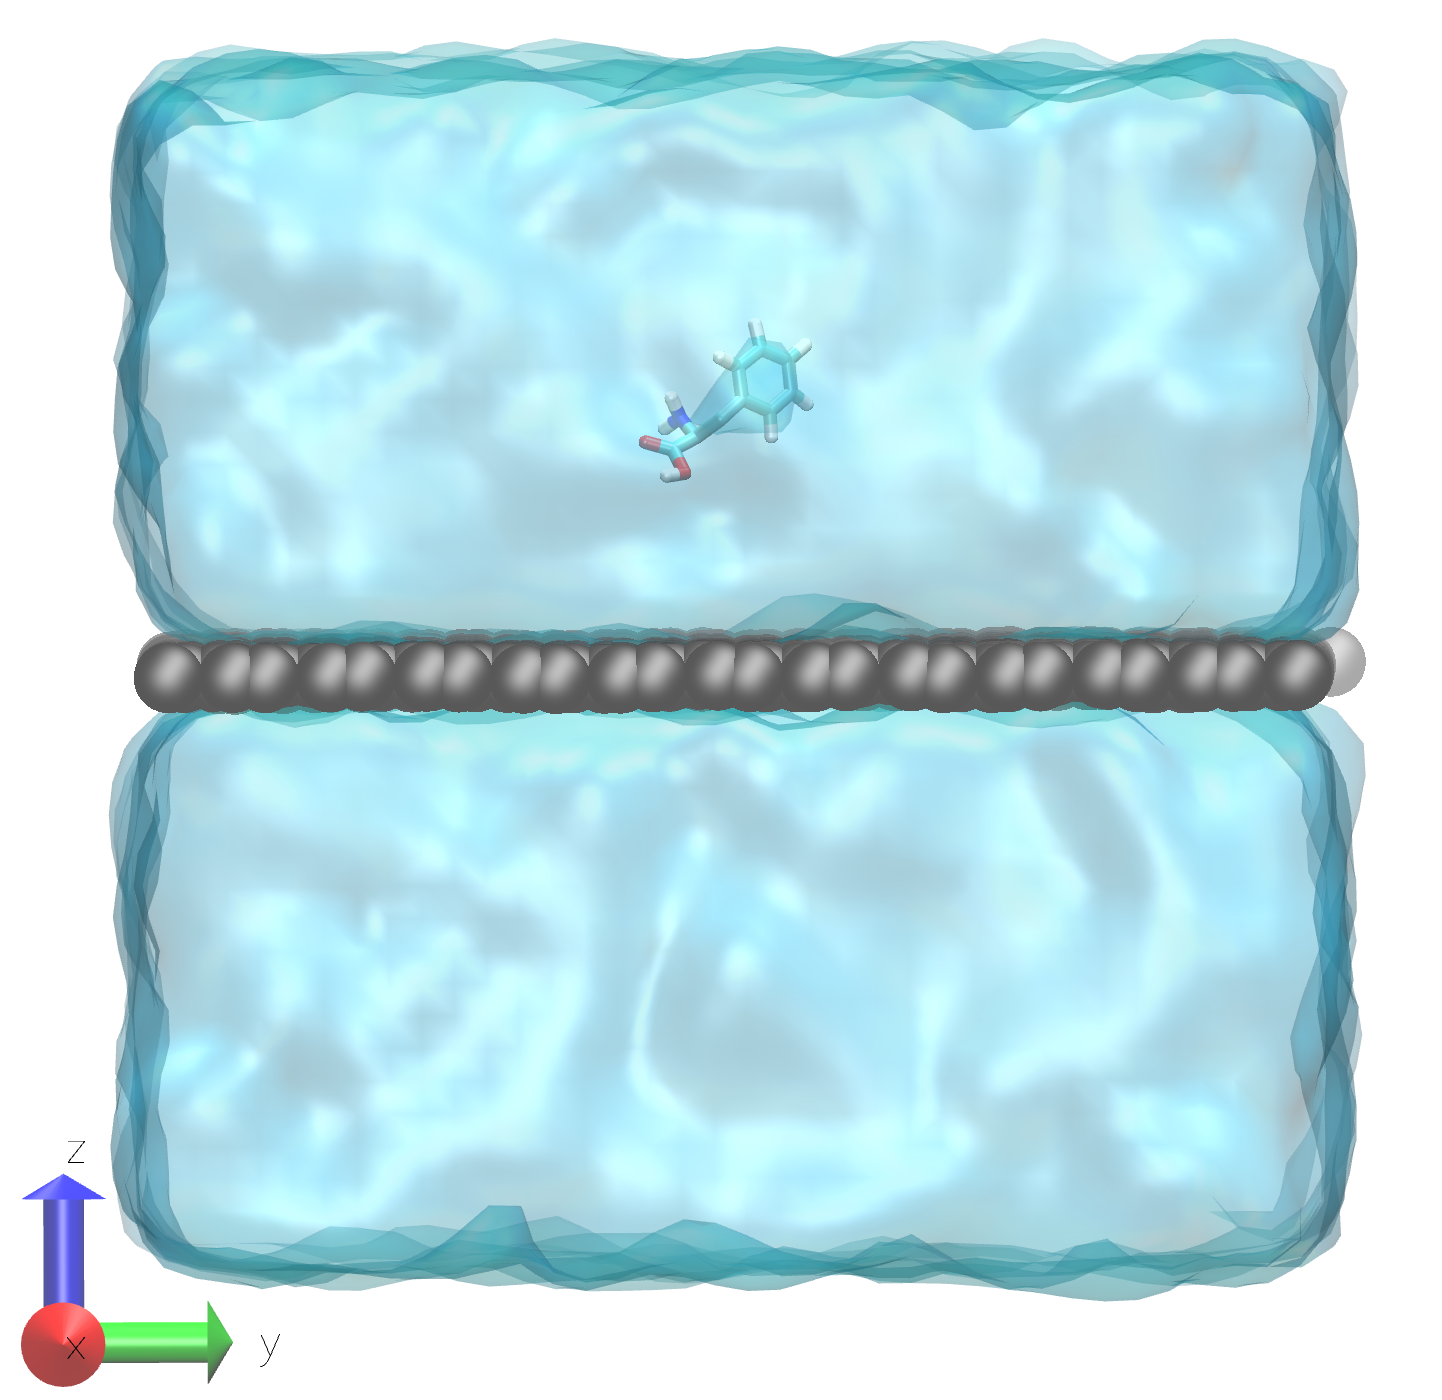
\includegraphics[width=\columnwidth]{/home/mbarria/Dropbox/Papers/graphene_adsorption_paper/figures/Pristine_System.png}}
\caption[]{\label{fig:system-pristine} Example of simulated pristine
  graphene systems. An amino acid (in this case Phenylalanine) above a
  graphene layer (in gray) inside a periodic water box.}
\end{figure}

\begin{figure}[htbp]
\centerline{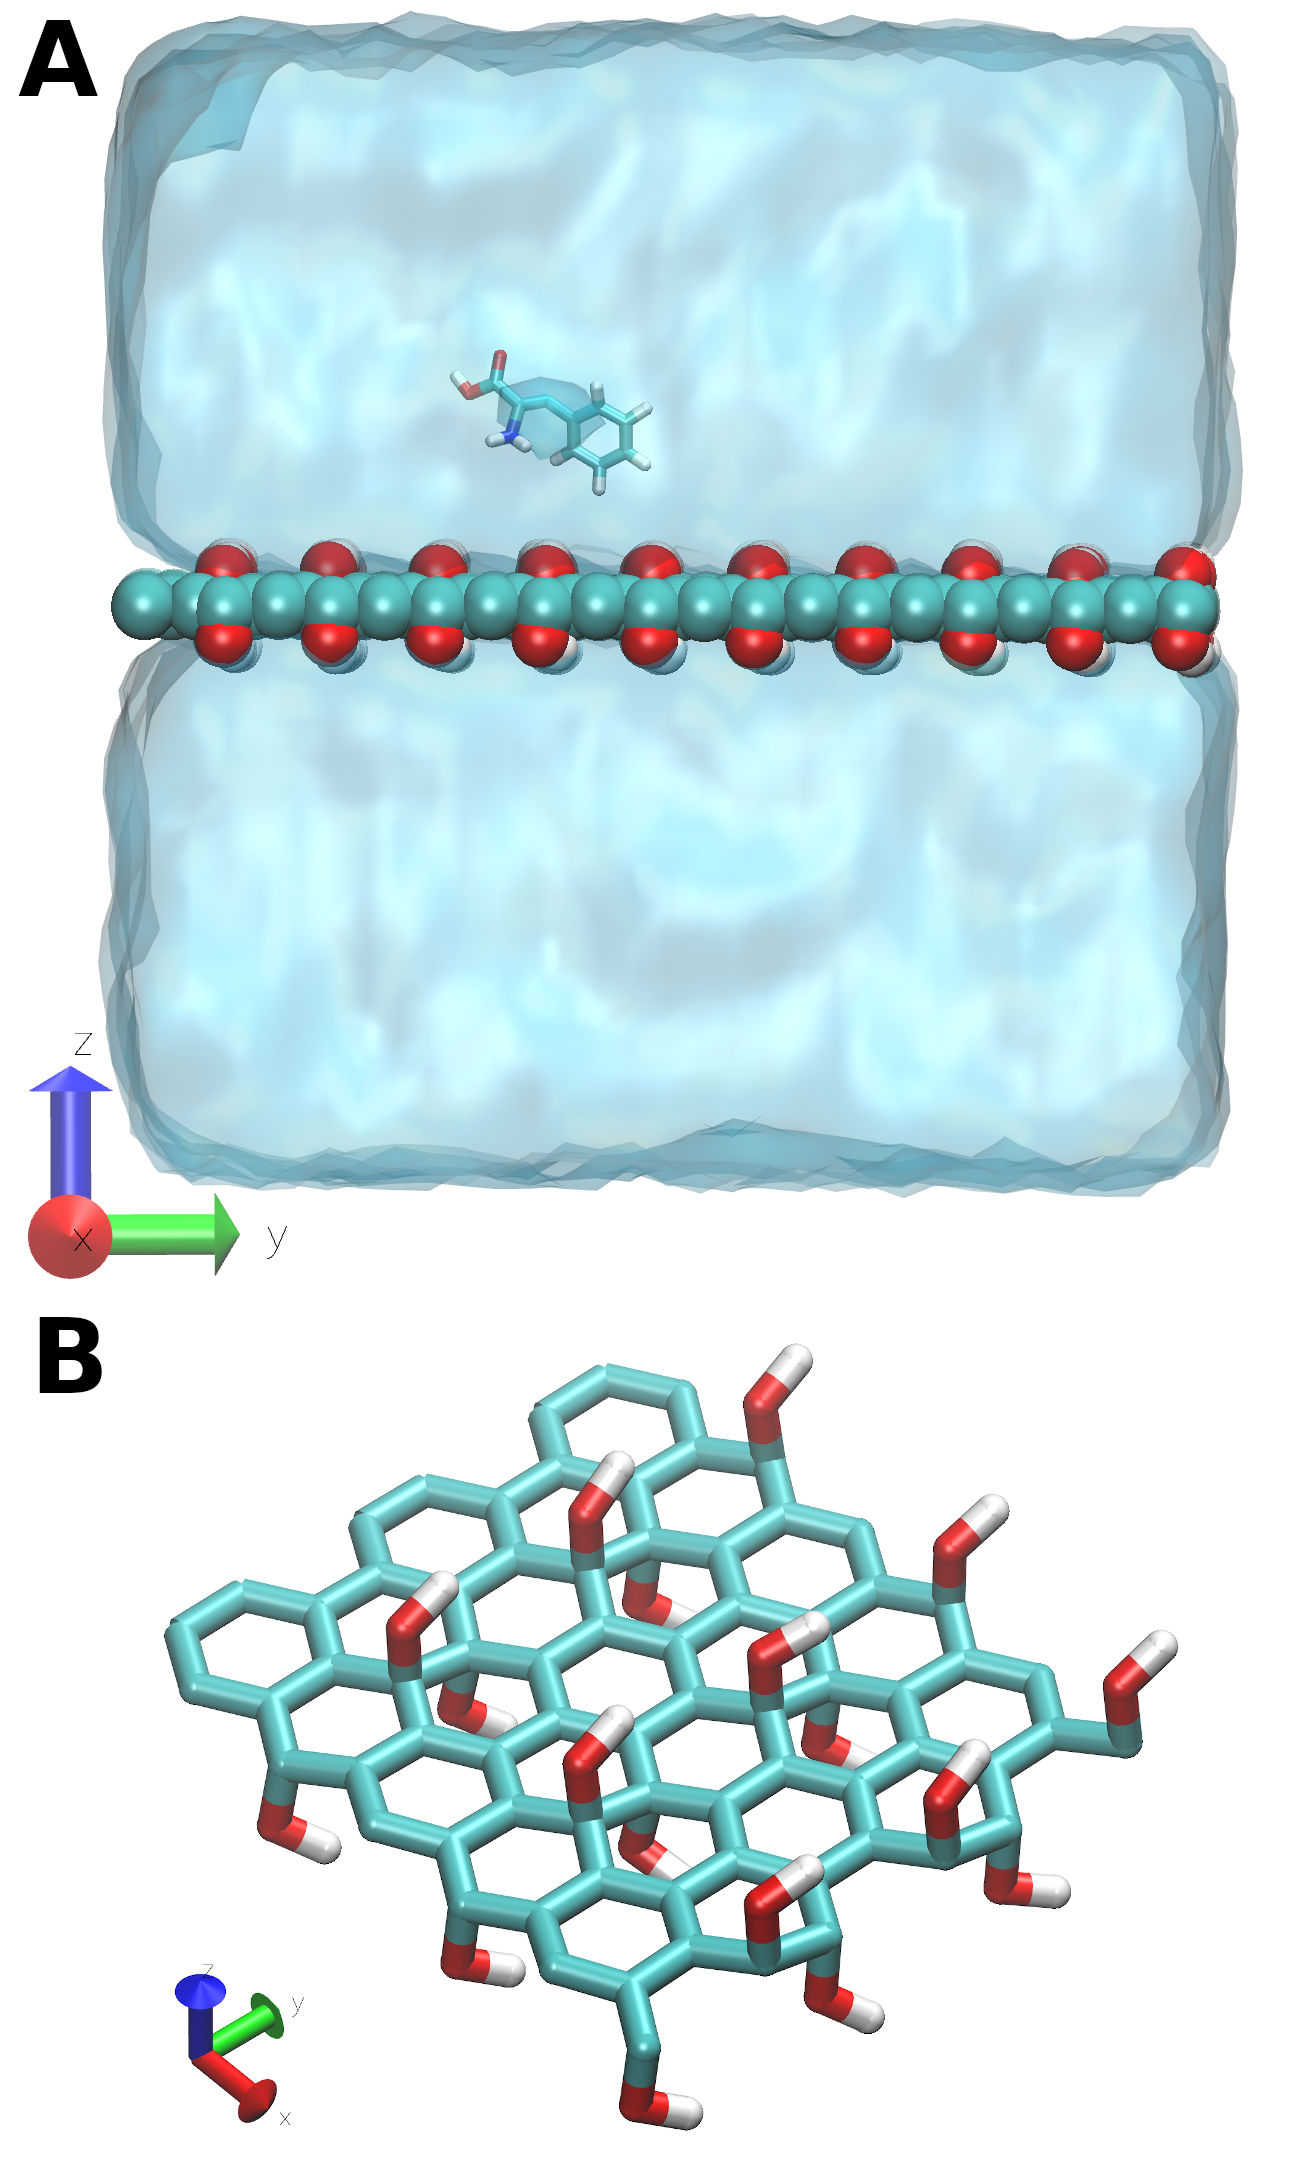
\includegraphics[width=\columnwidth]{/home/mbarria/Dropbox/Papers/graphene_adsorption_paper/figures/Oxidized_System_and_Unit.png}}
\caption[]{\label{fig:system-oxidized} a) Example of simulated oxidized
  graphene systems. An amino acid (in this case Phenylalanine) above a
  graphene layer (C in gray, O in red, H in white) inside a periodic
  water box. b) Segment of the oxidized graphene layer depicting the
  oxidation pattern. (C in gray, O in red, H in white)}
\end{figure}

MD simulations were performed using the GROMOS11 \cite{Riniker_2011,
  Schmid_2012} and the NAMD 2.14 simulation packages
\cite{Phillips_2020}.  Details of the simulations will be presented
separately for each program.

\subsubsection{GROMOS}

The SHAKE algorithm \cite{Ryckaert_1977} was employed to constrain all
bonds to their reference values with a relative tolerance of
$10^{-4}$, allowing for a time-step of 2 fs using the leapfrog
algorithm \cite{Hockney_1977}.  For water, the SPC model was used
\cite{Berendsen_1981}.  Non-bonded interactions were computed using a
triple range cut-off. Interactions within the short-range cut-off of
0.8 nm were computed every time-step, from a pair-list that was
generated every 5 steps.  At these time points, interactions between
0.8 and 1.4 nm were also computed which were kept constant between
these updates.  A reaction-field contribution was added to
electrostatic interactions approximating for a homogeneous medium
outside the 1.4 nm long-range cut-off, employing the relative
permittivity of SPC water (61) \cite{Tironi_1995}. All interactions
were calculated using the GROMOS 54a8 potential energy function, with
all graphene atoms modeled as neutral sp$^2$ carbons \cite{Reif_2012}.
After a steepest-descent minimization to remove bad contacts, all
velocities were randomly assigned from a Maxwell-Boltzmann
distribution at 298 K.  All simulations were run coupled to
thermostats using the weak-coupling algorithm
\cite{Berendsen_1984}. The solute, graphene and solvent atoms were
independently coupled to different heat baths. Additionally, the
graphene layer was coupled to separate baths for regulation of its
center of mass motion and its rotational and internal degrees of
freedom. This totaled 4 heat baths.

Graphene sheets with sides of length $4.94$ and $4.87$ nm and
bond-length of $0.139$ nm were generated with VMD\cite{Humphrey_1996}
using its nanotube builder plugin.

\begin{figure}[htbp]
\centerline{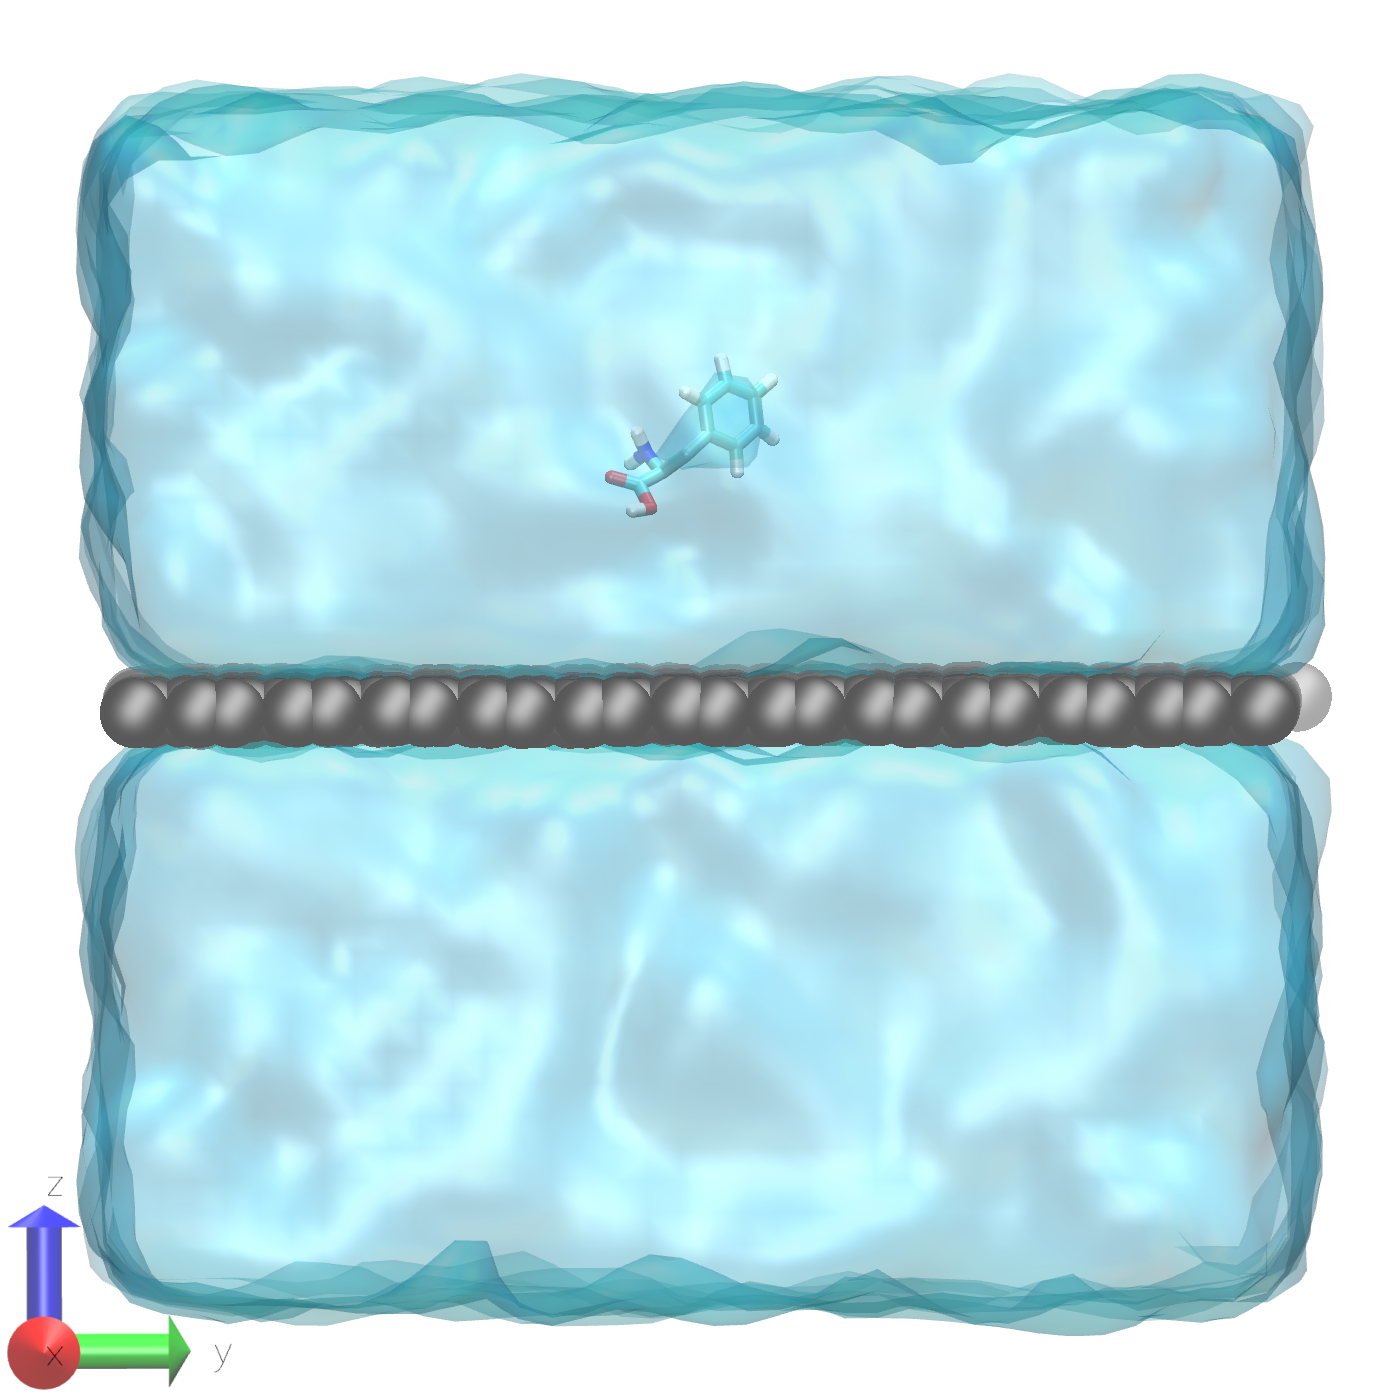
\includegraphics[width=\columnwidth]{/home/mbarria/Documents/Papers/graphene_adsorption_paper/figures/Graphene.png}}
\caption[]{\label{fig:system-pristine} Example of a simulated
  system. A Phenylalanine molecule is placed above a layer of pristine
  graphene inside a water-filled rectangular box. Carbon atoms are
  depicted in gray.}
\end{figure}

\begin{figure}[htbp]
\centerline{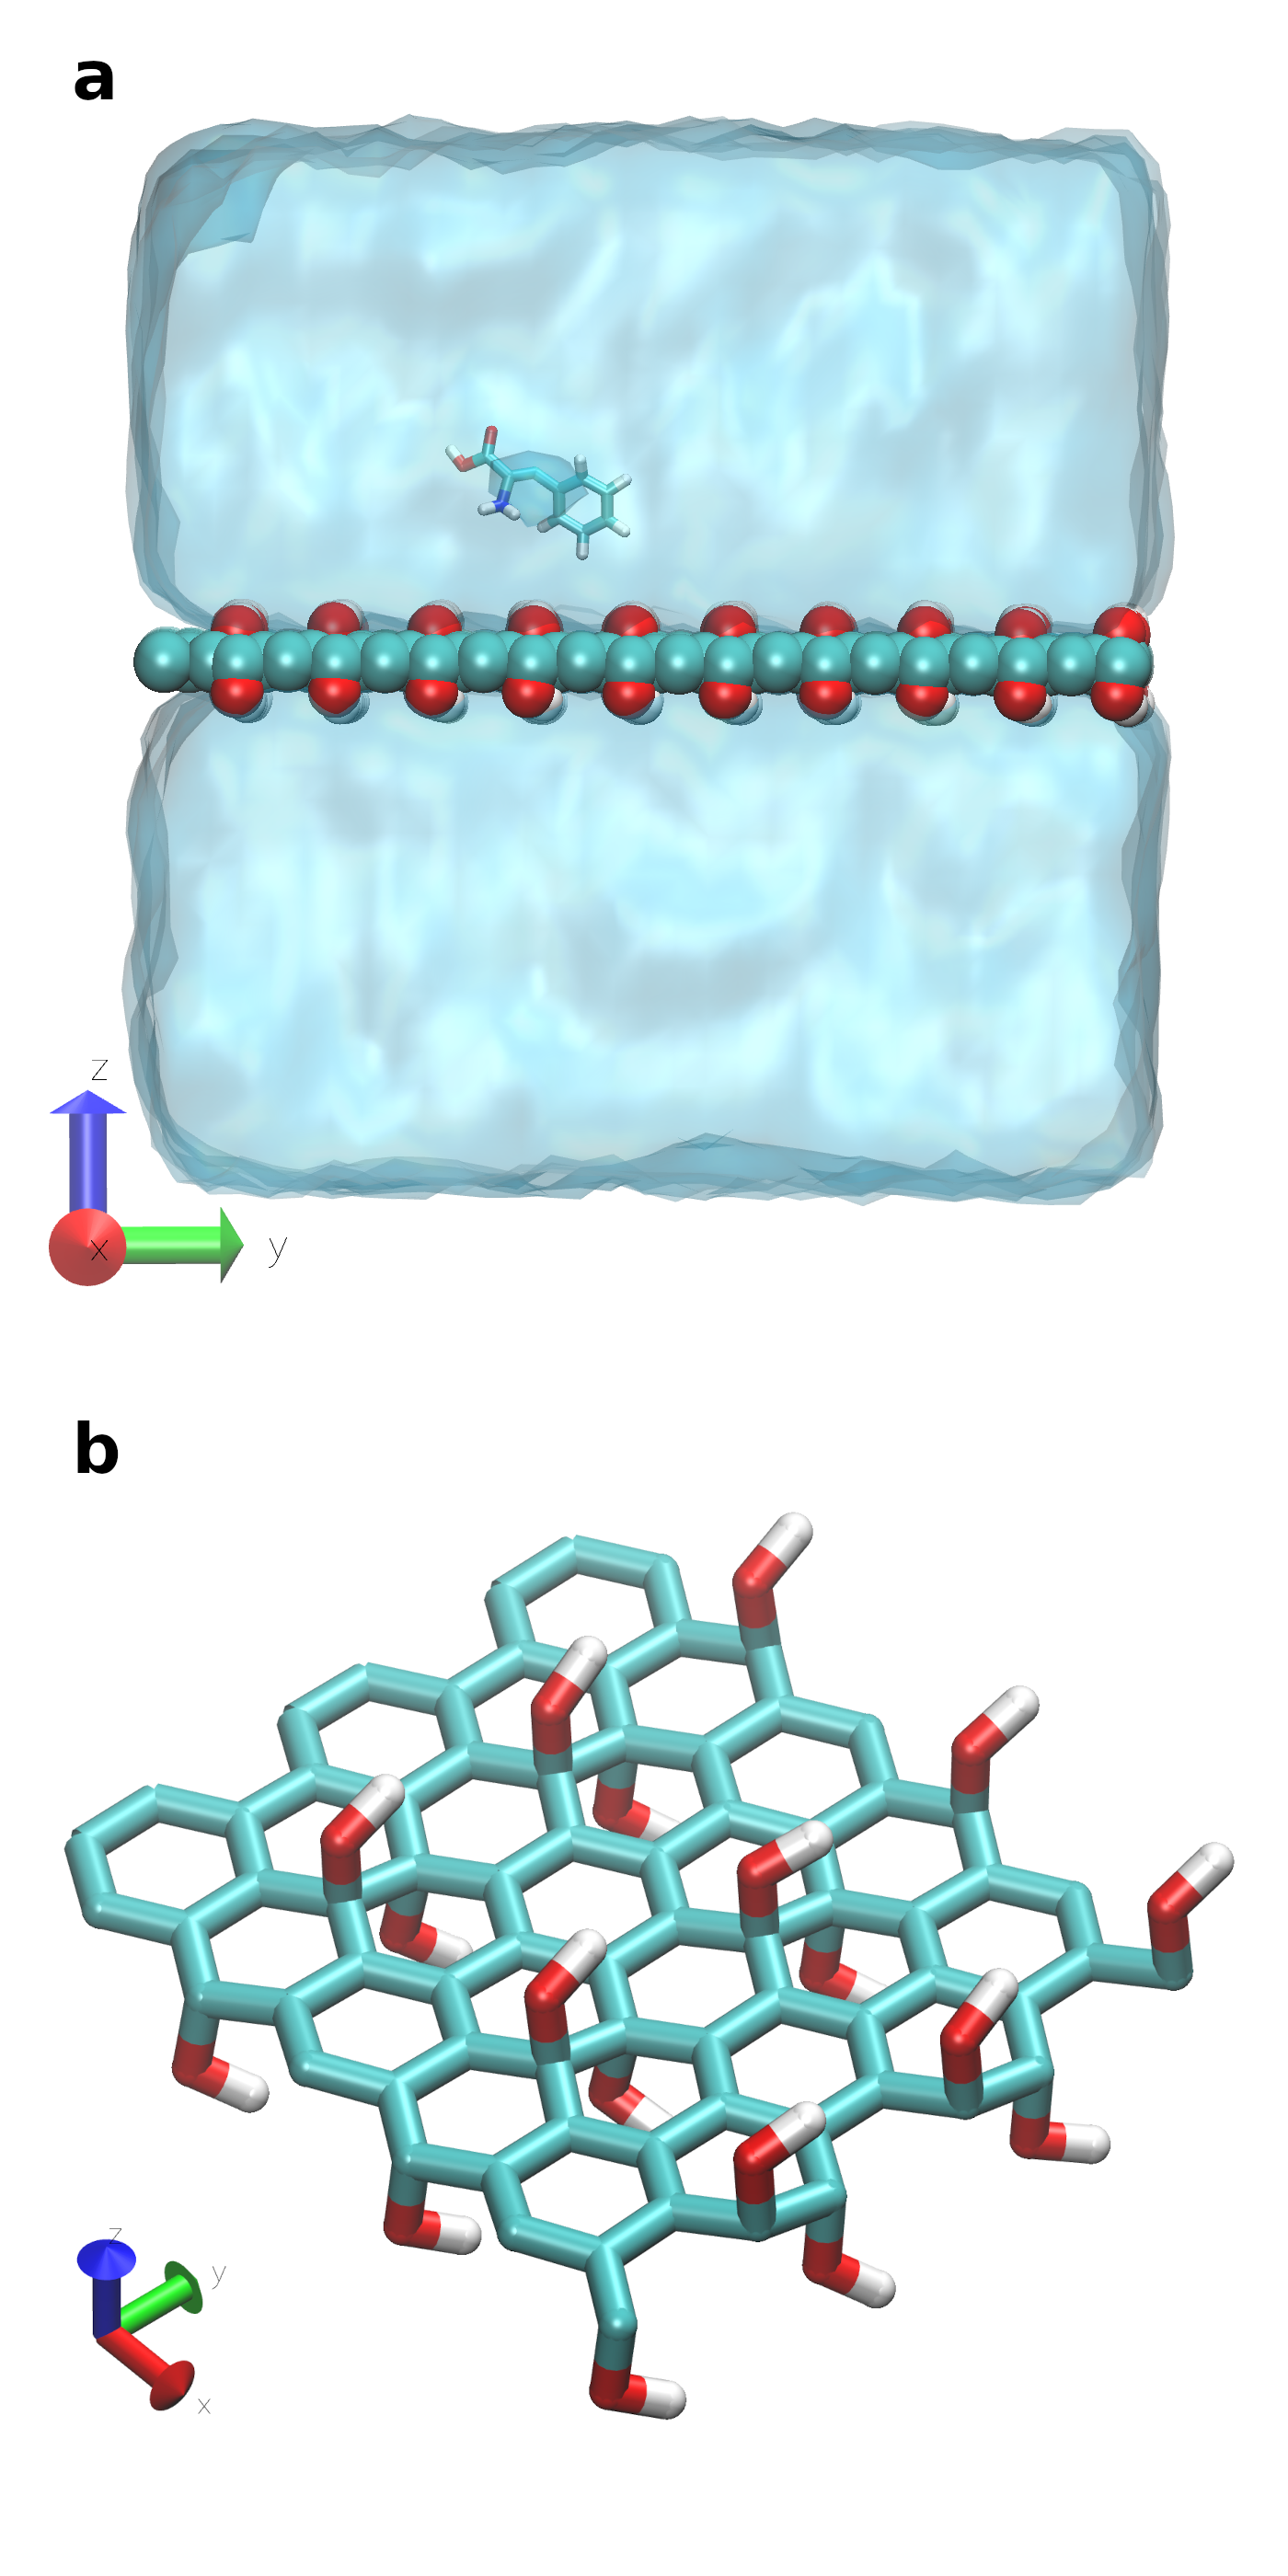
\includegraphics[width=\columnwidth]{/home/mbarria/Documents/Papers/graphene_adsorption_paper/figures/Graphene_Oxide.png}}
\caption[]{\label{fig:system-oxide} (a) A simulated system where the
  graphene layer is oxidized. Carbon atoms are depicted in cyan, while
oxygen and hydrogen atoms are depicted in red and white,
respectively. (b) A section of the graphene oxide layer, showing the
distribution of the hydroxyl groups.}
\end{figure}

% \subsection{Quantum Mechanics / Molecular Mechanics}
% NAMD was used for QM/MM simulations due to it's hybrid simulation
% implementation \cite{Melo_2018}


\section{Results}

\begin{figure*}[htbp]
\centerline{\includegraphics[width=\textwidth]{/home/mbarria/Dropbox/Papers/graphene_adsorption_paper/figures/Differences_by_names_and_weight.png}}
\caption[]{\label{fig:differences} Differences of adsorption over a
  pristine graphene layer for free energies ($\Delta A_{ads}$),
  energies ($\Delta E_{ads}$) and entropies ($T \Delta S_{ads}$) for
  all proteinogenic amino acids. Top row (a, c, and e):
  $\Delta A_{ads}$, $\Delta E_{ads}$, and $T \Delta S_{ads}$, arranged
  by amino acid classification on the basis of side-chain
  interactions. Amino acids are labeled on the x-axis by their three
  letter code. Bottom row (b, d, and f): $\Delta A_{ads}$,
  $\Delta E_{ads}$, and $T \Delta S_{ads}$, as a function of molecular
  weight of the amino acid. Amino acids are labeled by their markers
  with their one letter code. In all cases amino acids are in a
  neutral state unless marked with a positive ($+$) or negative ($-$)
  sign.}

\end{figure*}

\begin{figure*}[htbp]
\centerline{\includegraphics[width=\textwidth]{/home/mbarria/Dropbox/Papers/graphene_adsorption_paper/figures/Differences_by_names_and_weight_25o.png}}
\caption[]{\label{fig:differences} Differences of adsorption over an
  oxidized graphene layer for free energies ($\Delta A_{ads}$),
  energies ($\Delta E_{ads}$) and entropies ($T \Delta S_{ads}$) for
  select amino acids. All values are relative to Glycine's, which is
  set to 0. Top row (a, c, and e): $\Delta A_{ads}$,
  $\Delta E_{ads}$, and $T \Delta S_{ads}$, arranged by amino acid
  classification on the basis of side-chain interactions. Amino acids
  are labeled on the x-axis by their three letter code. Bottom row (b,
  d, and f): $\Delta A_{ads}$, $\Delta E_{ads}$, and
  $T \Delta S_{ads}$, as a function of molecular weight of the amino
  acid. Amino acids are labeled by their markers with their one letter
  code. In all cases amino acids are in a neutral state unless marked
  with a positive ($+$) or negative ($-$) sign.}

\end{figure*}

\subsection{Adsorption Free Energy}

\subsection{Adsorption Entropy}

\subsection{Adsorption Energy}

\subsection{Diffusion}

\section{Conclusions}


\section*{Acknowledgements}
This work was partially supported by grant no. ICM-Economia grant
no. P09-022-F Centro Interdisciplinario de Neurociencia de Valparaiso,
Universidad de Valparaiso; FONDECYT 1180987 (to J.A.G.), PAI grant
no. 77170045 (to J.A.G.) and a doctoral scholarship from
CONICYT--PFCHA/DOCTORADO BECAS NACIONAL/2020--21201020.  Access to the
supercomputing infrastructure of the National Laboratory for
High-Performance Computing was supported through grant no. ECM-02
(Powered@NLHPC).


\bibliography{refs.bib}
\bibliographystyle{plainnat}

\end{document}

%%%Local Variables:
%%% mode: latex
%%% TeX-master: t
%%% End:
